\chapter{Quantum Repetition Code}\label{ch:quantum_repetition}

\section{Classical Repetition Code}
\label{sec:classical_repetition_code}

Suppose a noisy channel exists in which a bit flips with a probability $p$ \citep{Nielsen2010}. This implies that we will obtain the correct information with a probability of only $(1 - p)$. We can achieve better results by encoding the information. In this case, let us consider taking a single bit of information and encoding it into three bits. A particular aspect of this model is that every bit in the resulting sequence holds the same amount of information. This is a strictly classical concept known as \textit{redundancy} \citep{Nielsen2010}.

\begin{equation}
  \begin{aligned}
    1 &\to 111\\
    0 &\to 000
  \end{aligned}
  \label{img_1}
\end{equation}

After passing through the channel, we obtain a new bit string, which for the sake of this example we will call $S_n$. This string could match the original or result in any other combination of the three bits, depending on the number of errors that occurred. Decoding is where the primary advantages of using a code become apparent. In this example, there are two main decoding methods to improve fidelity \citep{Nielsen2010}:

\begin{enumerate}
\item We could implement a majority-vote system, meaning we interpret the bit string as representing bit 0 if the majority of the bits are 0, and similarly for 1 \citep{Nielsen2010}.
\item Alternatively, we can check if pairs of bits are equal. This detects whether an error occurred and indicates how to correct it. In this specific scenario, one can compare the first bit with the second, and the first bit with the third \citep{Nielsen2010}.
\end{enumerate}

These two systems function essentially the same way within classical computing theory. However, the first method cannot be directly translated into quantum computing because it requires measuring each qubit independently. Therefore, we will focus on the second option for the decoding process to draw a direct parallel with the quantum equivalent of this code \citep{Nielsen2010}.

For ease of understanding, consider the case where the decoding process receives the bit string 010. In this scenario, the decoding procedure indicates that the first and second bits are different, while the first and third bits are equal, implying that the second bit was the source of the error \citep{Nielsen2010}.

However, that assumption could be incorrect; it is entirely possible that the first and third bits were the ones affected by the error. This indistinguishability between the two possibilities demonstrates that this code only works effectively if an error occurs in at most one bit. Consequently, the probability of an error remaining uncorrected with this code is \citep{Nielsen2010}:

\begin{equation}
p^3 + 3p^2(1 - p) = 3p^2 - 2p^3
.\end{equation}

\begin{figure}[H]
\centering
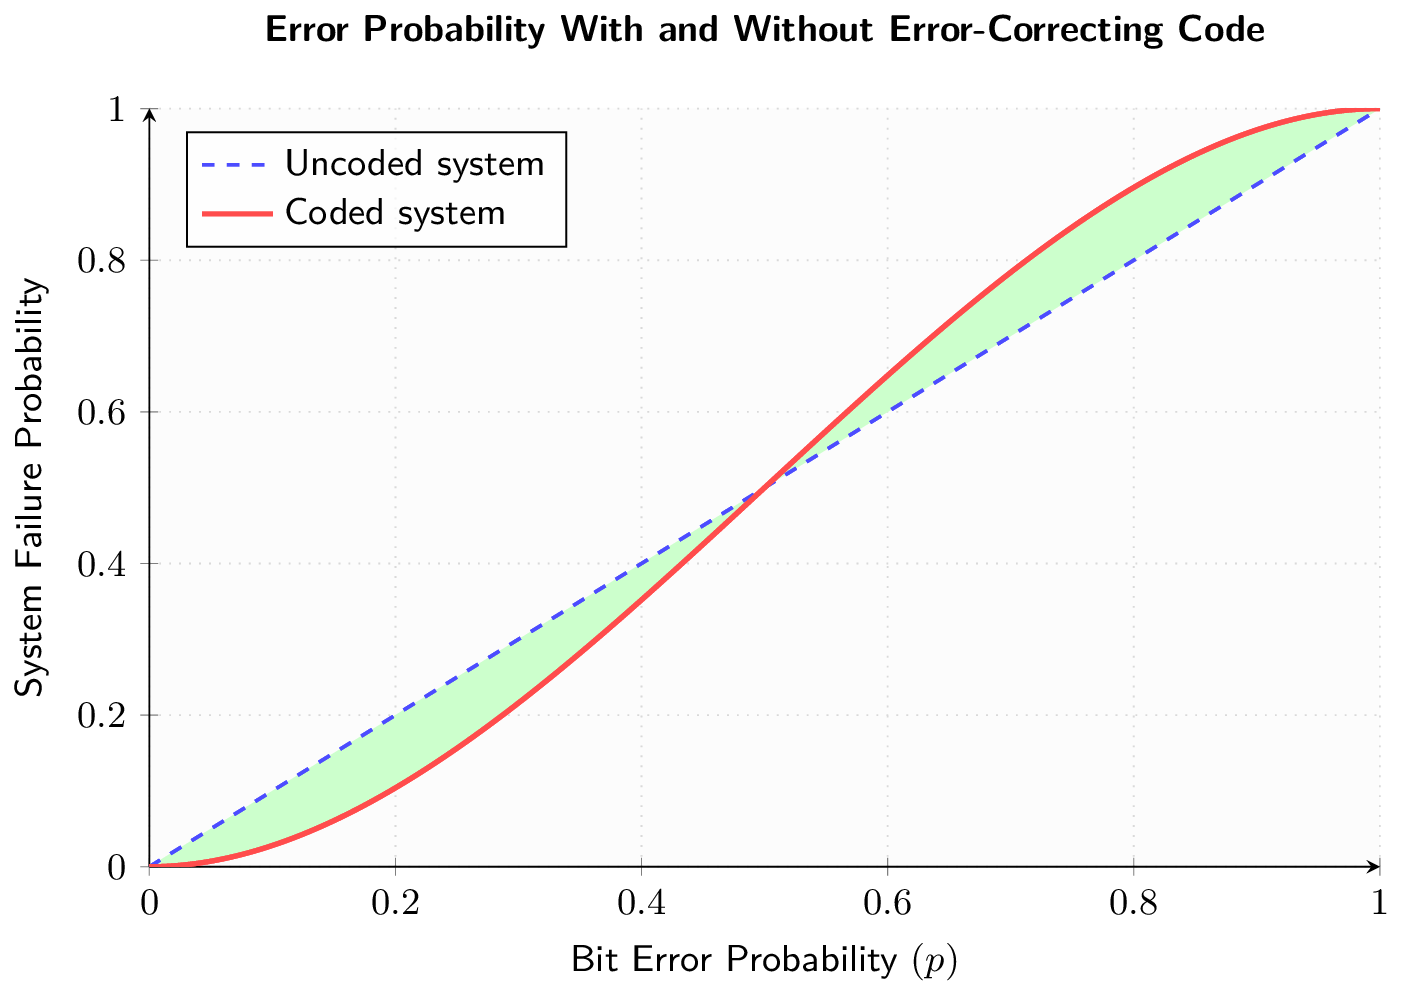
\includegraphics[width=0.7\linewidth]{files/02_comparison-2d9e0d455373d64bb1d46105fb84b631.png}
\caption{Comparison of the error probability for a bit transmitted through the channel with and without the code \citep{Nielsen2010}. The dashed blue line represents the unprotected bit, whose error probability is linear. The red line represents the encoded system, which performs better when the physical error probability is less than 50\%.}
\label{img_2}
\end{figure}

Note that without encoding, the probability of failure is simply $p$. Therefore, this code is only helpful if $3p^2 - 2p^3 \le p$, which holds exclusively when $p \le \frac{1}{2}$ \citep{Nielsen2010}. One can increase the number of bits used to encode the same information to obtain different thresholds of utility---a topic extensively studied in classical coding theory. Nevertheless, the core idea of encoding information is already captured by this three-bit example \citep{Nielsen2010}.

% TODO: ¿Debo agregar una sección haciendo los cálculos para un sistema de votación arbitrario para $n$ bits? Podría ser interesante.

\section{Quantum Repetition Code}

Having reviewed the classical repetition code in Section~\ref{sec:classical_repetition_code}, we can now transition to its quantum counterpart. This code relies on essentially the same theoretical principle. However, the decoding process must be interpreted through a different lens: we cannot duplicate identical information across multiple qubits due to quantum constraints. Instead, the information is distributed across all three qubits \citep{Nielsen2010}.

The first defining characteristic of this code is its encoding process. In a classical code, a bit can simply be copied; however, this is impossible in quantum computing due to the no-cloning theorem. Nonetheless, we can construct a unitary operator that encodes a single logical qubit into three physical qubits, as illustrated by the circuit in Figure~\ref{quantum_repetition_code_encode_circuit} \citep{Nielsen2010}.

\begin{figure}[!htbp]
\centering
\begin{quantikz}
\lstick{$\ket{\psi}$} & \ctrl{1} & \ctrl{2} & \qw \\
\lstick{$\ket{0}$}     & \targ{}  & \qw      & \qw \\
\lstick{$\ket{0}$}     & \qw      & \targ{}  & \qw
\end{quantikz}
\caption{Circuit that encodes a single qubit in a manner equivalent to the classical repetition code. This demonstrates that encoding is possible due to the existence of a linear, unitary process \citep{Nielsen2010}.}
\label{quantum_repetition_code_encode_circuit}
\end{figure}

Once encoded, the logical codespace is defined by the following projector \citep{Nielsen2010}:

\begin{equation}
P = \ket{000}\bra{000} + \ket{111}\bra{111}
.\end{equation}

The decoding process, as demonstrated previously, is divided into two stages. First, we extract the error syndrome, which is achieved by applying the following projectors \citep{Nielsen2010}:

\begin{itemize}
\item $P_0 = \ket{000}\bra{000} + \ket{111}\bra{111}$ (No error occurred)
\item $P_1 = \ket{100}\bra{100} + \dots + \ket{011}\bra{011}$ (Error in the first qubit)
\item $P_2 = \ket{010}\bra{010} + \dots + \ket{101}\bra{101}$ (Error in the second qubit)
\item $P_3 = \ket{001}\bra{001} + \dots + \ket{110}\bra{110}$ (Error in the third qubit)
\end{itemize}

Second, we correct the error by applying the appropriate recovery operation based on the syndrome obtained. This approach is analogous to the classical problem; therefore, the fidelity analysis is identical and yields equivalent results \citep{Nielsen2010}.

Furthermore, because this is a quantum code, we can explicitly demonstrate its ability to correct bit-flip errors using the Knill-Laflamme conditions \citep{Nielsen2010}. Given our previously defined projector $P$ and the set of single-qubit bit-flip error operators:

\begin{equation}
\{E_i\} = \left\{I \otimes I \otimes I, X \otimes I \otimes I, I \otimes X \otimes I, I \otimes I \otimes X \right\}
.\end{equation}

We can now verify that the Knill-Laflamme conditions hold for this code. First, considering the cases where $i = j$ (since $E_i^\dagger E_i = I$ for Pauli matrices), the condition reduces to:
\begin{align*}
  P E_i^\dagger E_i P &= P I P \\
  &= P^2 \\
  &= P
.\end{align*}
Therefore, $\alpha_{ii} = 1$. Conversely, for $i \neq j$, applying the error operators to the projector $P$ yields $P_{ij}$, which is the original operator modified by the application of $E_i$ and $E_j^\dagger$. This resulting operator is orthogonal to the original projector, meaning $\alpha_{ij} = 0$. In summary, the matrix $\alpha$ is the identity matrix, which is Hermitian, as required \citep{Nielsen2010}.

\subsection{Limitations with Arbitrary Errors}

Let us consider the standard phase-basis states \citep{Nielsen2010}:

\begin{equation}
  \ket{+} = \frac{\ket{0} + \ket{1}}{\sqrt{2}};\quad \ket{-} = \frac{\ket{0} - \ket{1}}{\sqrt{2}}
  \label{eq:hadamard_phase}
.\end{equation}

Now, suppose the operations $I$ and $Z$ are applied exclusively to the first qubit as the errors for the Knill-Laflamme conditions. Focusing solely on the first qubit, we observe that \citep{Nielsen2010}:

\begin{align*}
  \braket{-|+} &= 0 \\
  \bra{-}I^{\dagger}Z\ket{+} &= \braket{-|-} \neq 0
.\end{align*}

Consequently, it is impossible to correct phase-flip errors using this specific repetition code \citep{Nielsen2010}.
